\documentclass[11pt,a4paper]{article}
\usepackage[T1]{fontenc}
\usepackage[margin=2.3cm]{geometry}
\usepackage{amsmath,amssymb}
\usepackage{graphicx}
\usepackage[dvipsnames]{xcolor}
\usepackage{enumitem}
\usepackage[colorlinks=true,linkcolor=blue,urlcolor=blue]{hyperref}
\setlength{\parskip}{0.6em}
\setlength{\parindent}{0pt}
\begin{document}

\begin{center}{\LARGE\bfseries openwatershed}\\[0.4em]{\large Predict how high a river rises when it rains, in three sessions.}\\[0.2em]\small PAN IIT OSS explainer \textbullet{} secondary school to diploma / undergraduate (levels 3-5)\end{center}

\section*{Why this exists}
When it rains on a valley, some water soaks in and the rest runs to the river. This explainer shows the mathematics that turns rainfall into a flood peak, using only arithmetic, a little algebra and convolution, so you can build it yourself.

\section*{The end goal}
Predict a river's flood peak from rainfall on a watershed. The end goal is predicting a river's flood peak from rainfall on a watershed, as hydrologists do with run-off recipes and unit hydrographs. All models here are simplified teaching models: real flood forecasts and designs come from official agencies and qualified hydrologists.

\section*{How the three sessions build up}
\begin{enumerate}[nosep]
\item \textbf{Session 1: From rain to river} (Level 1, conceptual interactive model, 60 min).
\item \textbf{Session 2: Two standard recipes: rational method and curve number} (Level 2, mathematical engineering model, 75 min).
\item \textbf{Session 3: The unit hydrograph, urbanisation and a detention pond} (Level 3, simulation and validation, 90 min).
\end{enumerate}

\section{Session 1: From rain to river}

\subsection*{A. Real-world problem}
A storm drops the same 60 mm of rain on the hills above a town twice: once in 1 hour, once spread over 6 hours. In which case does the river rise higher? The answer decides how high a bridge or a flood wall must be. This lesson is a simplified teaching model: real flood forecasts come from official agencies and qualified hydrologists.

\subsection*{B. Concept and theory}
The ground can swallow water at a rate f (mm per hour), like a sponge. Rain that falls faster than f cannot soak in, so the excess runs off over the surface. Run-off is a depth rate (mm/h) spread over the catchment area A (km2); 1 mm of water over 1 km2 is 1000 m3, so 1 mm/h over 1 km2 is 1000 m3 per hour = 0.2778 m3/s, and flow in m3/s is depth rate times area divided by 3.6. The water does not reach the river at once: it trickles down slopes and gullies. The simplest picture is a tank with a leak (a linear reservoir) with delay K: if the run-off flow is q for D hours, the river flow rises as q(1 - exp(-t/K)), reaches q(1 - exp(-D/K)) at the end of the storm, then falls away. A storm much shorter than K never lets the river reach q, which is why a long gentle storm of the same depth gives a smaller peak.

\begin{itemize}[nosep]
\item P: total storm rain depth (mm)
\item D: storm duration (h)
\item i = P / D: rain intensity (mm/h)
\item f: soak-in rate of the ground (mm/h)
\item A: catchment area (20 in this lesson) (km2)
\item K: catchment delay (2 in this lesson) (h)
\item q: run-off flow (m3/s)
\item Q\_peak: river peak flow (m3/s)
\end{itemize}

\begin{equation*}
\text{run-off rate}=\max(i-f,\,0)\qquad i=P/D
\end{equation*}

\begin{equation*}
q=\frac{\max(i-f,0)\,A}{3.6}\quad\left(\tfrac{\text{mm}}{\text{h}}\cdot\text{km}^2\to\text{m}^3/\text{s}\right)
\end{equation*}

\begin{equation*}
Q(t)=q\left(1-e^{-t/K}\right)\ (t\le D),\qquad Q_{\text{peak}}=q\left(1-e^{-D/K}\right)
\end{equation*}

\begin{equation*}
Q(t)=Q_{\text{peak}}\,e^{-(t-D)/K}\ (t>D)
\end{equation*}

\begin{center}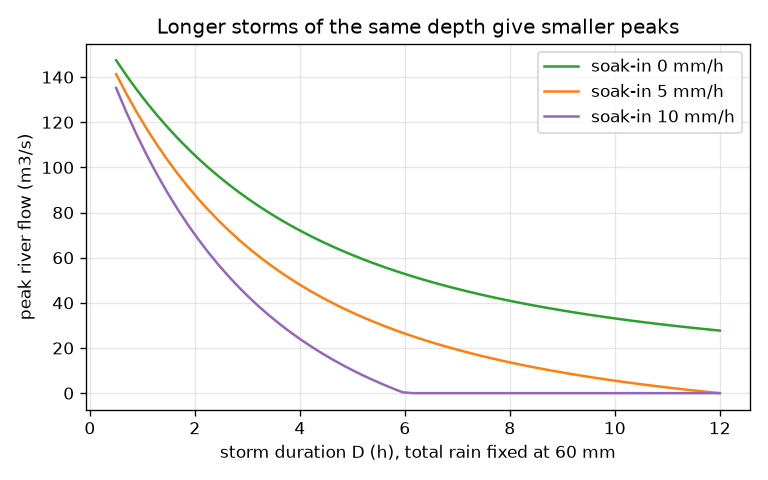
\includegraphics[width=0.85\linewidth]{figures/s01_peak_vs_duration.png}\\\small Peak river flow against storm duration for three soak-in rates.\end{center}

\subsection*{E. Worked example}
60 mm of rain falls in 1 h on a 20 km2 catchment with f = 5 mm/h and K = 2 h. Find the run-off flow and the river peak. Then do the same for 60 mm in 6 h.
\begin{enumerate}[nosep]
\item Intensity i = 60 / 1 = 60 mm/h. Run-off rate = 60 - 5 = 55 mm/h.
\item Flow q = 55 * 20 / 3.6 = 305.6 m3/s.
\item Peak = 305.6 * (1 - exp(-1/2)) = 305.6 * 0.3935 = 120.2 m3/s.
\item 6 h storm: i = 10 mm/h, run-off rate 5 mm/h, q = 5 * 20 / 3.6 = 27.78 m3/s.
\item Peak = 27.78 * (1 - exp(-6/2)) = 27.78 * 0.9502 = 26.4 m3/s.
\item Run-off volumes: 55 mm gives 1100 thousand m3 and 30 mm gives 600 thousand m3 over the 20 km2.
\end{enumerate}
\textbf{Answer.} The short storm gives a peak of 120.2 m3/s and the long one 26.4 m3/s: more than four times lower for the same 60 mm of rain.

\subsection*{F. Questions}
\begin{enumerate}[nosep]
\item \textbf{Conceptual.} Why can a storm with less total rain sometimes cause a bigger flood than a storm with more rain?
\item \textbf{Numerical.} 60 mm of rain falls in 2 h on the 20 km2 catchment (f = 5 mm/h, K = 2 h). Find the river peak and check the units.
\item \textbf{Graph and simulation interpretation.} In the graph of peak against duration (rain fixed at 60 mm), what do the 0 and 10 mm/h curves tell you at D = 6 h? What happens as D gets small?
\item \textbf{Design and optimisation challenge.} Design: land use changes can raise f from 5 to 10 mm/h (for example, more open soil and trees). For the 60 mm, 1 h storm, does that bring the peak below 100 m3/s? What else would you change, and what do you assume?
\end{enumerate}

\section{Session 2: Two standard recipes: rational method and curve number}

\subsection*{A. Real-world problem}
A culvert (a pipe under a road) must carry the flood of a small stream, Mango Creek (made up): 4.5 km2, a longest flow path of 3200 m and a drop of 64 m. Engineers need two numbers: how much of a storm becomes run-off (a depth, in mm) and how big the flow peak is (m3/s). Two classic recipes give them. Pipe hydraulics is in openpipeflow and structures in openretainingwall; here we stop at the flow in the stream. Educational model, not a design tool.

\subsection*{B. Concept and theory}
Rational method: Q = C i A / 3.6, with C the run-off coefficient (0 to 1, the share of the rain that runs off), i the rain intensity (mm/h), A the area (km2) and Q the peak flow (m3/s). The factor 3.6 is a unit conversion: 1 mm/h over 1 km2 is 1000 m3/h = 0.2778 m3/s. SCS curve number: soil and cover are summarised by CN (higher means more run-off). S = 25400/CN - 254 is the most water the ground can still hold (mm), Ia = 0.2 S is the rain lost at the start (the 0.2 is a standard approximation), and the run-off depth is Q = (P - Ia)\textasciicircum{}2 / (P - Ia + S) when P \textgreater{} Ia, otherwise zero. As P grows, Q/(P - Ia) tends to 1 and the water kept after Ia tends to S. Time of concentration Tc is the time water needs from the farthest point to the outlet; the Kirpich formula (metric, approximate, for small rural catchments) is Tc = 0.0195 L\textasciicircum{}0.77 S\textasciicircum{}-0.385 minutes with L in metres and S the slope (drop over length). The design storm lasts Tc: a shorter storm is more intense but only part of the catchment has delivered yet, a longer one is gentler, so the peak is best at D = Tc. We model the contributing area as A min(1, D/Tc), a simple approximation, with a made-up rain intensity curve i = 2000/(t + 15) for a storm of t minutes.

\begin{itemize}[nosep]
\item Q (rational): peak flow (m3/s)
\item C: run-off coefficient (no unit)
\item i: rain intensity (mm/h)
\item A: catchment area (km2)
\item CN: curve number (no unit)
\item S: maximum retention (mm)
\item Ia: initial loss (mm)
\item P: storm rain depth (mm)
\item Q (SCS): run-off depth (mm)
\item L, S\_slope: flow path length (m) and slope (m/m) (m, no unit)
\item Tc: time of concentration (min)
\end{itemize}

\begin{equation*}
Q=\frac{C\,i\,A}{3.6}\qquad \frac{1\,\text{mm/h}\times 1\,\text{km}^2}{1}=\frac{10^3\,\text{m}^3}{3600\,\text{s}}=0.2778\,\text{m}^3/\text{s}
\end{equation*}

\begin{equation*}
S=\frac{25400}{CN}-254,\qquad I_a=0.2\,S
\end{equation*}

\begin{equation*}
Q=\frac{(P-I_a)^2}{P-I_a+S}\ (P>I_a),\qquad Q=0\ (P\le I_a)
\end{equation*}

\begin{equation*}
T_c\approx 0.0195\,L^{0.77}\,S_{\text{slope}}^{-0.385}\ \text{(min; } L \text{ in m)}
\end{equation*}

\begin{center}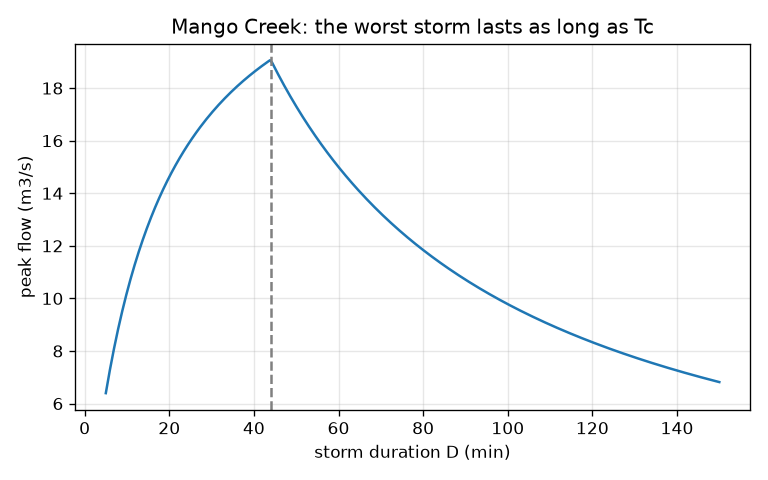
\includegraphics[width=0.85\linewidth]{figures/s02_peak_vs_duration.png}\\\small Mango Creek: the peak is largest when the storm lasts as long as Tc (about 44 min).\end{center}

\subsection*{E. Worked example}
Mango Creek (A = 4.5 km2) gets a 100 mm storm; CN = 80. Find S, Ia, the run-off depth and volume. Then estimate Tc, the design intensity and the rational peak with C = 0.45.
\begin{enumerate}[nosep]
\item S = 25400/80 - 254 = 317.5 - 254 = 63.5 mm. Ia = 0.2 * 63.5 = 12.7 mm.
\item P - Ia = 87.3 mm. Q = 87.3\textasciicircum{}2 / (87.3 + 63.5) = 7621.3 / 150.8 = 50.54 mm.
\item Volume = 0.05054 m * 4.5 km2 = 0.05054 * 4 500 000 m2 = about 227 thousand m3.
\item Slope = 64 / 3200 = 0.02. Tc = 0.0195 * 3200\textasciicircum{}0.77 * 0.02\textasciicircum{}-0.385 = 44.0 min.
\item Intensity for a 44 min storm: i = 2000 / (44.0 + 15) = 33.9 mm/h (made-up curve).
\item Rational peak = 0.45 * 33.9 * 4.5 / 3.6 = 19.1 m3/s.
\end{enumerate}
\textbf{Answer.} Run-off depth 50.54 mm (about 227 thousand m3), Tc about 44 min, rational peak about 19.1 m3/s.

\subsection*{F. Questions}
\begin{enumerate}[nosep]
\item \textbf{Conceptual.} Why does the SCS curve give zero run-off for small storms, and why does Q stay below P for every storm?
\item \textbf{Numerical.} A 60 mm storm falls on Mango Creek with CN = 75. Find the run-off depth and the volume over 4.5 km2.
\item \textbf{Graph and simulation interpretation.} On the run-off graph, at what storm depth does the CN 60 curve leave zero, and the CN 90 curve? What does the difference mean?
\item \textbf{Design and optimisation challenge.} Design: a plan straightens the channel of Mango Creek so that the slope doubles (0.02 to 0.04). Compute the new Tc and rational peak (C = 0.45, same area) and say whether the downstream culvert needs to be bigger. What do you assume?
\end{enumerate}

\section{Session 3: The unit hydrograph, urbanisation and a detention pond}

\subsection*{A. Real-world problem}
A stream gauge shows a curve, the hydrograph, not a single number. A real storm has bursts, and each makes its own little flood. Then a developer paves part of a 12 km2 valley (made up). How much higher and earlier is the new peak, and how large a pond holds it back to the old value? Educational model only: real flood studies use gauged data, official rainfall and qualified hydrologists.

\subsection*{B. Concept and theory}
Effective rain: the SCS run-off of the cumulative rain, differenced burst by burst. Unit hydrograph (UH): the response to 1 mm of effective rain in one burst of length D. The SCS triangular form (standard, approximate) has time to peak Tp = D/2 + 0.6 Tc, peak Qp = 0.208 A Pe / Tp (A in km2, Pe in mm, Tp in h, Qp in m3/s) and base time 2.67 Tp; the 0.208 follows from requiring the area under the triangle to equal 1 mm over A, i.e. 1000 A m3. Convolution: burst k with effective rain Pe[k] adds Pe[k] times the UH, shifted by k steps, so Q[n] = sum over k of Pe[k] U[n-k]. Urbanisation raises CN (more run-off) and shortens Tc (faster water). Muskingum routing: O[n+1] = C0 I[n+1] + C1 I[n] + C2 O[n] with the weights below (they add to 1); it delays and flattens a flood wave while keeping its volume. Detention pond (level pool): the water balance Ap dh/dt = I(t) - O(h) for a vertical-walled pond of surface area Ap with an orifice O = c sqrt(h); c is chosen so that O equals the old peak at the full depth H. We integrate with RK4 and find the smallest area by bisection. For this pond only the volume Ap H matters, not the chosen depth. Limits: the model is lumped, uses an approximate triangular UH, a fixed CN, and a simple outlet.

\begin{itemize}[nosep]
\item Pe: effective (run-off) rain per burst (mm)
\item A: catchment area (12) (km2)
\item Tc: time of concentration (h)
\item D: burst length (0.5) (h)
\item Tp: time to peak of the UH (h)
\item Qp: UH peak per mm (m3/s)
\item U[n]: UH ordinates (m3/s per mm)
\item K, X: Muskingum travel time and weighting (h, no unit)
\item I, O: inflow and outflow (m3/s)
\item Ap, H, h: pond area, full depth, water depth (m2, m, m)
\end{itemize}

\begin{equation*}
T_p=\frac{D}{2}+0.6\,T_c,\qquad Q_p=\frac{0.208\,A\,P_e}{T_p},\qquad t_b=2.67\,T_p
\end{equation*}

\begin{equation*}
Q[n]=\sum_{k}P_e[k]\,U[n-k]\quad(\text{discrete convolution})
\end{equation*}

\begin{equation*}
O_{n+1}=C_0 I_{n+1}+C_1 I_n+C_2 O_n,\ \ C_0=\frac{-KX+\Delta t/2}{K(1-X)+\Delta t/2},\ C_1=\frac{KX+\Delta t/2}{K(1-X)+\Delta t/2},\ C_2=\frac{K(1-X)-\Delta t/2}{K(1-X)+\Delta t/2}
\end{equation*}

\begin{equation*}
A_p\frac{dh}{dt}=I(t)-O(h),\qquad O=c\sqrt{h},\qquad \sqrt{h}=\sqrt{h_0}-\frac{c\,t}{2A_p}\ (I=0)
\end{equation*}

\begin{center}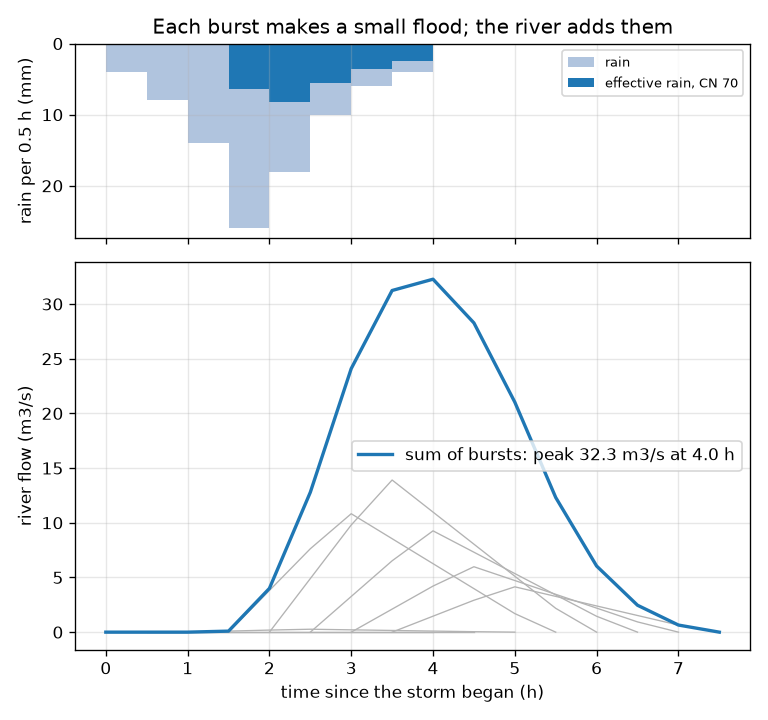
\includegraphics[width=0.85\linewidth]{figures/s03_convolution.png}\\\small The storm as bursts (top) and each burst's small flood in grey with their sum in blue.\end{center}

\subsection*{E. Worked example}
For the 12 km2 catchment, find the unit hydrograph for Tc = 2 h and D = 0.5 h, then the peaks before (CN 70, Tc 2.0 h) and after (CN 90, Tc 1.2 h) urbanisation, and the pond that restores the old peak.
\begin{enumerate}[nosep]
\item Tp = 0.5/2 + 0.6 * 2.0 = 1.45 h. Qp = 0.208 * 12 / 1.45 = 1.72 m3/s per mm. The UH holds 1 mm = 12 000 m3.
\item Effective rain of the 90 mm storm: 26.3 mm at CN 70 (the first hour of 12 mm is absorbed) and 63.2 mm at CN 90.
\item Convolve each burst with the UH and add: before, the peak is 32.3 m3/s at 4.0 h.
\item After (CN 90, Tc 1.2 h) the peak is 94.6 m3/s at 3.0 h: 2.9 times higher and 1 h earlier. The extra run-off volume is (63.2 - 26.3) mm * 12 km2 = 443 thousand m3.
\item Route the urbanised flood through a pond with an orifice that passes 32.3 m3/s at 2 m depth. Bisection gives a surface area of 226 857 m2, so the volume is about 454 thousand m3.
\item Checks: the outflow peak is 32.3 m3/s at 4.5 h, the water balance closes, and a pond half that size overtops (stage 3.31 m, outflow peak 41.5 m3/s).
\end{enumerate}
\textbf{Answer.} Peaks of 32.3 m3/s (before) and 94.6 m3/s (after); a pond of about 454 thousand m3 (226 857 m2 at 2 m) restores 32.3 m3/s, with the peak delayed to 4.5 h.

\subsection*{F. Questions}
\begin{enumerate}[nosep]
\item \textbf{Conceptual.} Why does the flood hydrograph equal the sum of shifted copies of the unit hydrograph, and what two assumptions make that valid?
\item \textbf{Numerical.} A catchment has A = 8 km2 and Tc = 1.5 h; the burst length is D = 0.5 h. Find Tp and the UH peak per mm. Check the 0.208 factor.
\item \textbf{Graph and simulation interpretation.} In the urbanisation figure, by how much do the peak and its time change, and which of the two changes (CN or Tc) matters more for the peak?
\item \textbf{Design and optimisation challenge.} Design: you can build the pond 1 m, 2 m or 3 m deep, with the orifice always passing 32.3 m3/s at the full depth. How does the required volume change, and what does a 1 m deep pond need in surface area? What trade-offs would you weigh?
\end{enumerate}

\section{Real-world mini-project}
\textbf{Urbanise a valley and size the detention pond.} A developer wants to pave part of the made-up 12 km2 catchment of Session 3: the curve number rises from 70 to 90 and the time of concentration falls from 2.0 h to 1.2 h. Using the shipped functions, compute the 90 mm storm hydrograph before and after, report the peaks and their times, then find the smallest pond volume that brings the peak back to the pre-development value. Use a pond with vertical walls and an orifice outlet that passes the old peak at a depth of 2 m.

\section{The path ahead}
\begin{enumerate}[nosep]
\item \textbf{Session 4: Design storms from a rainfall curve.} A function that builds a design storm of a chosen duration from an intensity curve and feeds it to the unit hydrograph.
\item \textbf{Session 5: A smoother unit hydrograph.} A second UH function with the same volume and a smooth rising limb.
\item \textbf{Session 6: Ponds with sloping banks and a spillway.} A level-pool router with a sloping-bank pond, an orifice and an overflow weir.
\item \textbf{Session 7: Two sub-catchments joined by a river.} A model that computes two sub-catchment hydrographs, routes one through Muskingum and adds them.
\item \textbf{Session 8: Calibrate against an observed flood.} A least-squares fit of CN and Tc to a synthetic observed hydrograph with added noise.
\end{enumerate}

\section{Answers and hints}

\subsection*{Session 1}
\begin{enumerate}[nosep]
\item \textbf{Conceptual.} Hint: Think about the two things that matter: how fast the rain arrives compared with the soak-in rate, and how long the catchment needs to gather the water. Solution: Run-off starts only when intensity exceeds the soak-in rate, and the river peak depends on how much run-off arrives within the delay time K. A short intense storm of modest depth can exceed f by a lot and deliver its water inside K, giving a high peak, while a long gentle storm of larger depth may stay near f and spread its water out. In this model, 60 mm in 1 h gives 120.2 m3/s but 60 mm in 6 h only 26.4 m3/s.
\item \textbf{Numerical.} Hint: i = P / D, then run-off rate, then flow = rate * area / 3.6, then multiply by 1 - exp(-D/K). Solution: i = 30 mm/h, run-off rate 25 mm/h, q = 25 * 20 / 3.6 = 138.9 m3/s, peak = 138.9 * (1 - exp(-1)) = 138.9 * 0.6321 = 87.8 m3/s. Units: mm/h * km2 / 3.6 gives m3/s. Sanity check: it lies between the 1 h answer (120.2) and the 6 h answer (26.4).
\item \textbf{Graph and simulation interpretation.} Hint: Read the curves at D = 6 and at the left edge of the graph. Solution: With no soak-in (0 mm/h) the 6 h storm gives a peak of 52.8 m3/s while with 10 mm/h it gives zero because the intensity (10 mm/h) does not exceed f. As D gets small the peak rises towards the ceiling set by the full intensity: with f = 0 the 1 h storm already gives 131.2 m3/s and with f = 5 the 0.5 h storm gives 141.3 m3/s. All curves fall as the storm lengthens.
\item \textbf{Design and optimisation challenge.} Hint: Compute the peak with f = 10 and compare with 100; then think about K and the storm duration. Solution: With f = 10 the 1 h peak is 109.3 m3/s, down from 120.2 but still above 100. Raising f helps only a little against an intense storm; storing water or slowing it (a larger K) would be needed. Assumptions: f is constant, the storm is even, and the catchment is one tank. A real designer uses official rainfall data and checks several storm durations.
\end{enumerate}

\subsection*{Session 2}
\begin{enumerate}[nosep]
\item \textbf{Conceptual.} Hint: What are Ia and S physically? Solution: The ground has to satisfy an initial loss Ia (hollows, wetting) before any water runs off, so for P at or below Ia there is no run-off. After that the ground keeps taking water, with the total kept after Ia tending to S, so Q is always smaller than P. Only CN = 100 (S = 0, roofs and water) sends all rain to run-off.
\item \textbf{Numerical.} Hint: S = 25400/75 - 254 = 84.7 mm; Ia = 0.2 S. Solution: S = 84.67 mm and Ia = 16.93 mm. P - Ia = 43.07 mm. Q = 43.07\textasciicircum{}2 / (43.07 + 84.67) = 14.52 mm. Volume = 0.01452 m * 4.5e6 m2 = 65.3 thousand m3. Units: mm of depth times km2 gives thousand m3.
\item \textbf{Graph and simulation interpretation.} Hint: Read off Ia = 0.2 S for each. Solution: CN 60 has Ia = 33.9 mm and CN 90 has Ia = 5.6 mm. Wetter, more paved land (CN 90) starts to run off after only 5.6 mm of rain, so even small storms flood it, while CN 60 land absorbs the first 33.9 mm. For 100 mm of rain the CN 60 land gives only 18.6 mm of run-off.
\item \textbf{Design and optimisation challenge.} Hint: Doubling the slope multiplies Tc by 2\textasciicircum{}-0.385; use the same intensity curve. Solution: Tc becomes 44.0 * 0.766 = 33.7 min, i = 2000 / (33.7 + 15) = 41.1 mm/h and the peak is 0.45 * 41.1 * 4.5 / 3.6 = 23.1 m3/s, about 21 percent more than 19.1 m3/s. So the culvert must carry more. Assumptions: Kirpich holds, C stays 0.45, the intensity curve is right; a designer must use official rainfall data and checks other storm durations.
\end{enumerate}

\subsection*{Session 3}
\begin{enumerate}[nosep]
\item \textbf{Conceptual.} Hint: Think about doubling the rain and about two bursts at different times. Solution: If the catchment responds linearly, twice the effective rain gives twice the flow (scaling), and two bursts at different times give the sum of their responses (superposition), shifted by the delay between them. That is exactly a discrete convolution. The assumptions are linearity and time invariance: the response does not depend on how wet the catchment is or on when the rain falls, which is only approximately true.
\item \textbf{Numerical.} Hint: Tp = D/2 + 0.6 Tc; Qp = 0.208 A / Tp. For the factor, 1000 / (0.5 * 2.67 * 3600). Solution: Tp = 0.25 + 0.9 = 1.15 h. Qp = 0.208 * 8 / 1.15 = 1.45 m3/s per mm. Check: 1000 / (0.5 * 2.67 * 3600) = 0.208, so the triangle with base 2.67 Tp holds 1 mm over A.
\item \textbf{Graph and simulation interpretation.} Hint: Compare the red curve with the blue one; the lesson also runs each change on its own. Solution: The peak rises from 32.3 to 94.6 m3/s (2.9 times) and comes 1 h earlier (4.0 h to 3.0 h). The curve number alone gives 76.0 m3/s at 3.5 h and a faster Tc alone gives only 39.3 m3/s at 3.0 h, so the larger run-off (CN) matters more for the size and the faster concentration mainly shifts the timing and adds the rest.
\item \textbf{Design and optimisation challenge.} Hint: Try size\_pond with different H and compare Ap * H. Solution: The volume stays the same (about 454 thousand m3) for all three depths, because in this vertical-wall model the dynamics depend only on the ratio of stored volume to capacity. A 1 m pond therefore needs about 454 thousand m2 (45 ha), a 2 m pond 227 thousand m2 and a 3 m pond 151 thousand m2. Trade-offs: deep ponds need less land but are a drowning hazard and need stronger embankments; shallow ponds use more land. A real design also needs a spillway for larger storms, and a qualified engineer.
\end{enumerate}

\section{How to join}
Read \texttt{CONTRIBUTING.md} in the repository, then pick an issue labelled \texttt{good first issue}. Repository: \url{https://github.com/KrunalPanchal1995/openwatershed}

\end{document}
